\begin{frame}{3D Cube}
\begin{center}
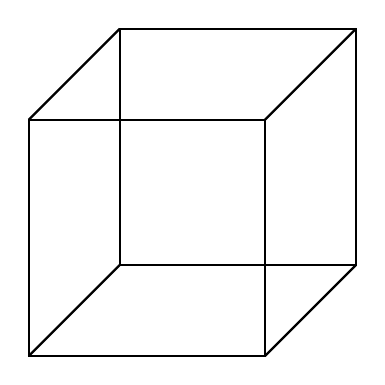
\begin{tikzpicture}[scale=1.5]
\draw[thick] (0,0,0) -- (2,0,0) -- (2,2,0) -- (0,2,0) -- cycle;
\draw[thick] (0,0,0) -- (0,0,2);
\draw[thick] (2,0,0) -- (2,0,2);
\draw[thick] (2,2,0) -- (2,2,2);
\draw[thick] (0,2,0) -- (0,2,2);
\draw[thick] (0,0,2) -- (2,0,2) -- (2,2,2) -- (0,2,2) -- cycle;
\end{tikzpicture}
\end{center}

\footnotesize
\texttt{\textbackslash draw[thick] (0,0,0) -- (2,0,0) -- (2,2,0) -- (0,2,0) -- cycle;}
\end{frame}